\section{Technologies utilisées}

\subsection{Java}

\par Java est un langage de programmation \textbf{orienté objet} développé par \textbf{Sun Microsystems} à partir de \textbf{1995}. La société sera plus tard rachetée par \textbf{Oracle} en 2009 qui possède et maintient Java encore aujourd'hui.
\par Java se détache de la masse des autres langages de programmation notamment grâce à sa portabilité et sa facilité d'utilisation.

\begin{lstlisting}[caption=Hello world en java]
public class HelloWorld {
    public static void main(String[] args) {
        System.out.println("Hello world!");
    }
}
\end{lstlisting}

Ci-dessus, un classique "Hello world" en Java. Nous pouvons y voir la définition de la classe \emph{HelloWorld} ainsi que la méthode principale du programme nommé \emph{main} et enfin un affichage sur la sortie standard.



\subsection{Le format MusicXML}
MusicXML est un format de fichier permettant de représenter la notation musicale occidentale (notation classique, accords en notation anglo-saxonne, tablatures et percussions) et basé sur le langage XML. Il est propriétaire mais il peut librement utilisé avec une licence publique.

Il y a plus de 20 ans, le format MIDI était très utilisé. Cependant, il n’est pas très adapté pour représenter toutes les caractéristiques de la musique, on perd donc en informations avec ce format. Pour pallier à cela, les formats SMDL et NIFF ont été créés. Cependant, le format SMDL était complexe et donc peu compréhensible. Il était donc très peu utilisé. Le format NIFF était un format peu pratique à utiliser et n’a donc pas été adopté par certains logiciels. Ces formats n’ont donc pas eu le succès souhaité.

En 2004, la société Recordare LLC s’inspire des 2 formats universitaires MuseData et Humdrum pour créer la première version du format MusicXML. Ses avantages sont qu’il est facile à manipuler. Il permet le transfert de morceaux de musique d’une application à une autre. Il peut représenter beaucoup de caractéristiques de la musique. Cependant, il est verbeux, puisqu'il utilise le format XML, et ne donc permet pas de représenter la musique non occidentale.

Il est de plus en plus utilisé puisque plus de 200 logiciels de musique l’ont adopté. Il est donc possible de travailler finement sur un morceau de musique en utilisant différents programmes. 

Comme le format XML est verbeux, le fichier prend de la place. La version 2.0, sortie en 2007, apporte donc la compression du fichier au format xml en un fichier au format mxl, et permet de diviser sa taille de façon importante. La version 3.0, sortie en 2011, permet le support des instruments virtuels.\\~\\

On voit, dans le code correspondant à la partition suivante, que les informations sur la partition sont placées dans la balise "measure" et celle concernant la ronde sont contenues dans la balise "note".

\begin{figure}[!h] %h : here
\centering
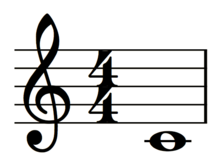
\includegraphics[width=0.2\textwidth]{musicxml_hello_world.png}\\[1cm]
%source : https://en.wikipedia.org/wiki/MusicXML
\caption{Hello World en MusicXML}
\label{Hello World en MusicXML}
\end{figure}

\newpage

\begin{lstlisting}[caption=Document XML d'un Hello World en MusicXML, label=ruleml]
<?xml version="1.0" encoding="UTF-8" standalone="no"?>
<!DOCTYPE score-partwise PUBLIC
    "-//Recordare//DTD MusicXML 3.0 Partwise//EN"
    "http://www.musicxml.org/dtds/partwise.dtd">
<score-partwise version="3.0">
  <part-list>
    <score-part id="P1">
      <part-name>Music</part-name>
    </score-part>
  </part-list>
  <part id="P1">
    <measure number="1">
      <attributes>
        <divisions>1</divisions>
        <key>
          <fifths>0</fifths>
        </key>
        <time>
          <beats>4</beats>
          <beat-type>4</beat-type>
        </time>
        <clef>
          <sign>G</sign>
          <line>2</line>
        </clef>
      </attributes>
      <note>
        <pitch>
          <step>C</step>
          <octave>4</octave>
        </pitch>
        <duration>4</duration>
        <type>whole</type>
      </note>
    </measure>
  </part>
</score-partwise>
\end{lstlisting}



\subsection{Le langage XML}

Le langage XML, acronyme de Extensible Markup Langage, est langage de balisage générique spécifié par le W3C. Il permet de définir différents espaces de noms, c'est à dire des langages avec leur propre grammaire et vocabulaire. Il permet l'échange d'information entre des programmes très différents à condition d'utiliser la même grammaire.

Il a l'avantage de pouvoir être compris par les êtres humains et les machines. Cependant, c'est un langage qui est verbeux et qui peut donc prendre beaucoup de place si il contient beaucoup d'information.

Un document XML est constitué de balises pouvant contenir d'autres balises ou une valeur simple. Une balise peut aussi contenir des attributs donnant des informations supplémentaires sur le contenu.

\begin{lstlisting}[caption=Exemple d'un document XML]
<?xml version="1.0" encoding="UTF-8"?>
<racine>
    <balise attribut="valeur" >Contenu</balise>
    <baliseunique />
</racine>
\end{lstlisting}

\par
Ci-dessus un exemple de XML simpliste mais qui met en avant les bases du langage. La première ligne annonce le type de document et la version dans lequel le document va être rédigé. \emph{<racine>} est le nœud racine du document, celui qui en somme va contenir tout le document. On peut ici, facilement remarquer que le document peut être représenté sous la forme d'un arbre.

\par
XML permet à l'utilisateur de définir lui même la grammaire de son document grâce notamment aux \textbf{DTD} et \textbf{XML Schema}. Ces outils nous permettent de disposer de format d’échange de données tel que \textbf{MusicXML}.


\subsection{Relax NG}
\textbf{Relax NG} (\textbf{Re}gular \textbf{La}nguage for \textbf{X}ML \textbf{N}ext \textbf{G}eneration) née de la fusion de TreX de James Clark et de Relax de Murata Makoto permet de définir la grammaire d'un document XML. Relax NG ne s'intéresse qu'à la structure de document et non leur valeur.
\par C'est ce que nous utiliserons afin de s'assurer de la validité du document à traiter.


\subsection{Affichage d'un graphe}
...

%mettre ici limage d'une partition et le graphe associé


\subsection{Les librairies}

Dans cette section, nous aborderons les librairies utilisé pour réaliser ce projet. Cela ira de la validation du XML en passant par le parsing de ce dernier jusqu'à la récupération des information stockées dans le fichier MusicXML.


\subsubsection{Trang et Jing}
\textbf{Trang} et \textbf{Jing} sont deux librairies développées par \textbf{Thai Open Source} permettant de générer des grammaire Relax NG et de valider des documents XML à partir de cette même grammaire.

Trang est une librairie qui permet de traduire un fichier de description grammaticale en fichier Relax NG. En effet XML n'est pas facilement lisible pour un esprit humain, c'est pour cela que Trang nous permet de créer notre grammaire dans un langage plus \emph{user-friendly}. Une fois la grammair écrite dans un fichier en \emph{.rnc}, nous pouvons générer notre fichier Relax NG en \emph{.rng}.

Jing, quant à lui, est une librairie Java qui permet de valider un document XML à l'aide d'un fichier Relax NG.

\begin{lstlisting}[caption=Code java permettant de vérifier la validation d'un document XML]

final ValidationDriver vd = new ValidationDriver();
vd.loadSchema(rngFile);

if (!vd.validate(inputTextStream)) {
	throw new ParseException("Invalid xml :(");
} else {
    System.out.println("Valid xml :)");
}
\end{lstlisting}

\par
Le code ci-dessus est une utilisation simplifié de Jing. Nous commençons tout d'abord par créer un \emph{ValidationDriver} de Jing dans lequel nous chargeons notre fichier Relax NG. Nous n'avons ensuite plus qu'à lancer la méthode \emph{validate(InputSource in) : boolean} qui nous indiquera si le document est valide.


\subsubsection{L'API SAX}

SAX est une API créée par David Megginson en 1998 et est l'acronyme de Simple API for XML. Elle permet de manipuler des documents XML en utilisant des événements.


\subsubsection{Le DOM}
Le DOM, ou Document Object Model, est une interface de programmation normalisée par le W3C et est indépendant de tout plateforme et langage. Il voit les documents à balises comme des arbres dont le contenu et la structure peuvent être accédés et mis à jour dynamiquement.

\begin{figure}[!h]
\centering
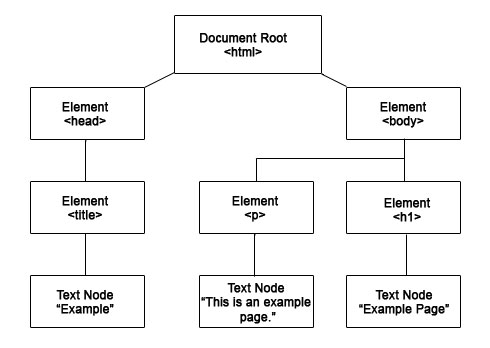
\includegraphics[width=0.8\textwidth]{ex_dom.jpg}\\[1cm]
%source : http://www.computerhope.com/jargon/d/dom.htm
\caption{Exemple d'un DOM}
\label{Exemple d'un DOM}
\end{figure}




